\documentclass[letterpaper,12pt]{article}
\usepackage{array}
\usepackage{threeparttable}
\usepackage{geometry}
\usepackage{float}
\geometry{letterpaper,tmargin=1in,bmargin=1in,lmargin=1.25in,rmargin=1.25in}
\usepackage{fancyhdr,lastpage}
\pagestyle{fancy}
\lhead{}
\chead{}
\rhead{}
\lfoot{}
\cfoot{}
\rfoot{\footnotesize\textsl{Page \thepage\ of \pageref{LastPage}}}
\renewcommand\headrulewidth{0pt}
\renewcommand\footrulewidth{0pt}
\usepackage[format=hang,font=normalsize,labelfont=bf]{caption}
\usepackage{listings}
\lstset{frame=single,
  language=Python,
  showstringspaces=false,
  columns=flexible,
  basicstyle={\small\ttfamily},
  numbers=none,
  breaklines=true,
  breakatwhitespace=true
  tabsize=3
}
\usepackage{amsmath}
\usepackage{amssymb}
\usepackage{amsthm}
\usepackage{harvard}
\usepackage{setspace}
\usepackage{float,color}
\usepackage[pdftex]{graphicx}
\usepackage{hyperref}
\hypersetup{colorlinks,linkcolor=red,urlcolor=blue}
\theoremstyle{definition}
\newtheorem{theorem}{Theorem}
\newtheorem{acknowledgement}[theorem]{Acknowledgement}
\newtheorem{algorithm}[theorem]{Algorithm}
\newtheorem{axiom}[theorem]{Axiom}
\newtheorem{case}[theorem]{Case}
\newtheorem{claim}[theorem]{Claim}
\newtheorem{conclusion}[theorem]{Conclusion}
\newtheorem{condition}[theorem]{Condition}
\newtheorem{conjecture}[theorem]{Conjecture}
\newtheorem{corollary}[theorem]{Corollary}
\newtheorem{criterion}[theorem]{Criterion}
\newtheorem{definition}[theorem]{Definition}
\newtheorem{derivation}{Derivation} % Number derivations on their own
\newtheorem{example}[theorem]{Example}
\newtheorem{exercise}[theorem]{Exercise}
\newtheorem{lemma}[theorem]{Lemma}
\newtheorem{notation}[theorem]{Notation}
\newtheorem{problem}[theorem]{Problem}
\newtheorem{proposition}{Proposition} % Number propositions on their own
\newtheorem{remark}[theorem]{Remark}
\newtheorem{solution}[theorem]{Solution}
\newtheorem{summary}[theorem]{Summary}
%\numberwithin{equation}{section}
\bibliographystyle{aer}
\newcommand\ve{\varepsilon}
\newcommand\boldline{\arrayrulewidth{1pt}\hline}
\graphicspath{{images/}}


\begin{document}

\begin{flushleft}
  \textbf{\large{Problem Set \#3}} \\
  MACS 30100, Dr. Evans \\
  Ningyin Xu
\end{flushleft}

\vspace{5mm}

\noindent\textbf{Problem 1. Some income data, lognormal distribution, and GMM.}

\noindent\textbf{Part (a).} 
\begin{figure}[htb]\centering\captionsetup{width=4.0in}
  \label{Fig1a}
  \fbox{\resizebox{4.0in}{3.0in}{
\includegraphics{Fig_1a.png}}}
\end{figure}
\\
\noindent\textbf{Part (b).} 
\begin{figure}[htb]\centering\captionsetup{width=4.0in}
  \label{Fig1b}
  \fbox{\resizebox{4.0in}{3.0in}{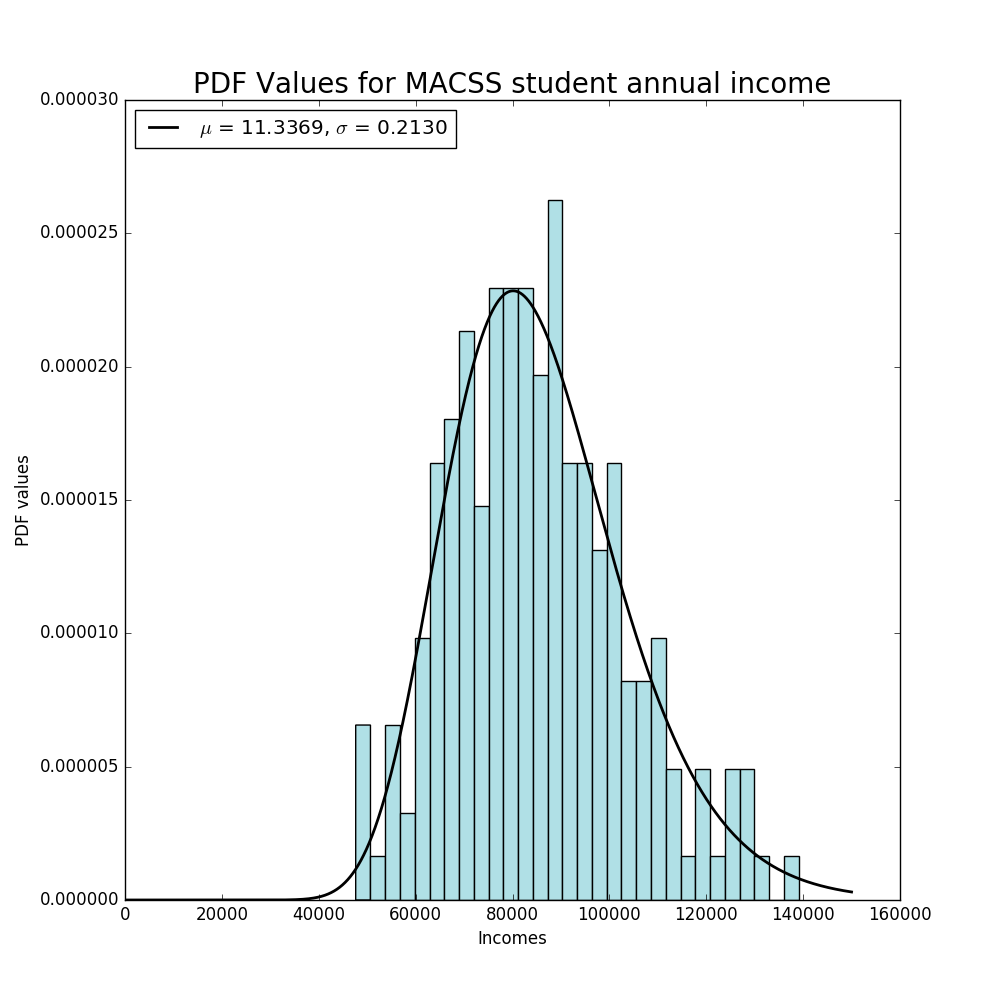
\includegraphics{Fig_1b.png}}}
\end{figure}
\newpage
\noindent
The value of GMM criterion function at the estimated parameter values is: $1.794297513712258e-13$.\\
And the data moments are: $\mu = 85276.8236$, $\sigma = 17992.5421$.\\
Model moments at the estimated parameter values are: $\mu = 85276.7904$, $\sigma = 17992.5391$.\\
They are pretty close, which means the GMM estimation performs well.\\
\\
\noindent\textbf{Part (c).}
\begin{figure}[htb]\centering\captionsetup{width=4.0in}
  \label{Fig1c}
  \fbox{\resizebox{4.0in}{3.0in}{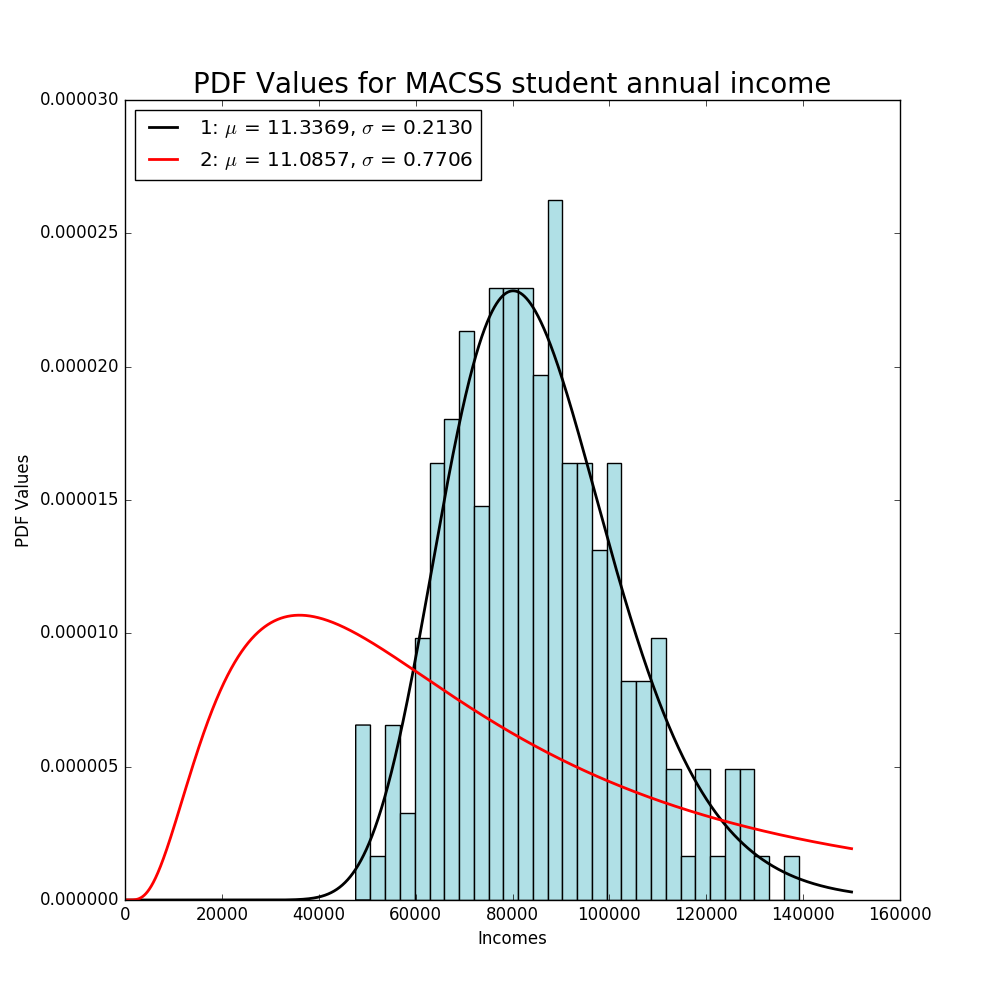
\includegraphics{Fig_1c.png}}}
\end{figure}
\\
The value of GMM criterion function at the estimated parameter values is: \\
$0.009984728414565325$.\\
And the data moments are: $\mu = 85276.8236$, $\sigma = 17992.5421$.\\
Model moments at the estimated parameter values are: $\mu = 54573.3360$, $\sigma = 33248.7952$.\\
Comparing to outcomes of part b, these model moments are less close to data moments.\\

\noindent\textbf{Part (d).}\\
\\
The value of GMM criterion function at the estimated parameter values is: \\
$2.534788361602213e-11$.\\
The three data moments are: \\
the proportion of individuals who earn less than \$75,000 is: $0.3$, \\
the proportion of individuals who earn more than \$75,000 but less than \$100,000 is: $0.5$, \\
the proportion of individuals who earn more than \$100,000 is: $0.2$. \\
The three model moments are: \\
the proportion of individuals who earn less than \$75,000 is: $0.30000000363261387$, \\
the proportion of individuals who earn more than \$75,000 but less than \$100,000 is: $0.5000000058562907$, \\
the proportion of individuals who earn more than \$100,000 is: $0.19999999051109518$.\\
I didn't take the rounding values here because I want to emphasize the difference, but you can tell these model moments are very close to data moments.\\
\begin{figure}[htb]\centering\captionsetup{width=4.0in}
  \label{Fig1d}
  \fbox{\resizebox{4.0in}{3.0in}{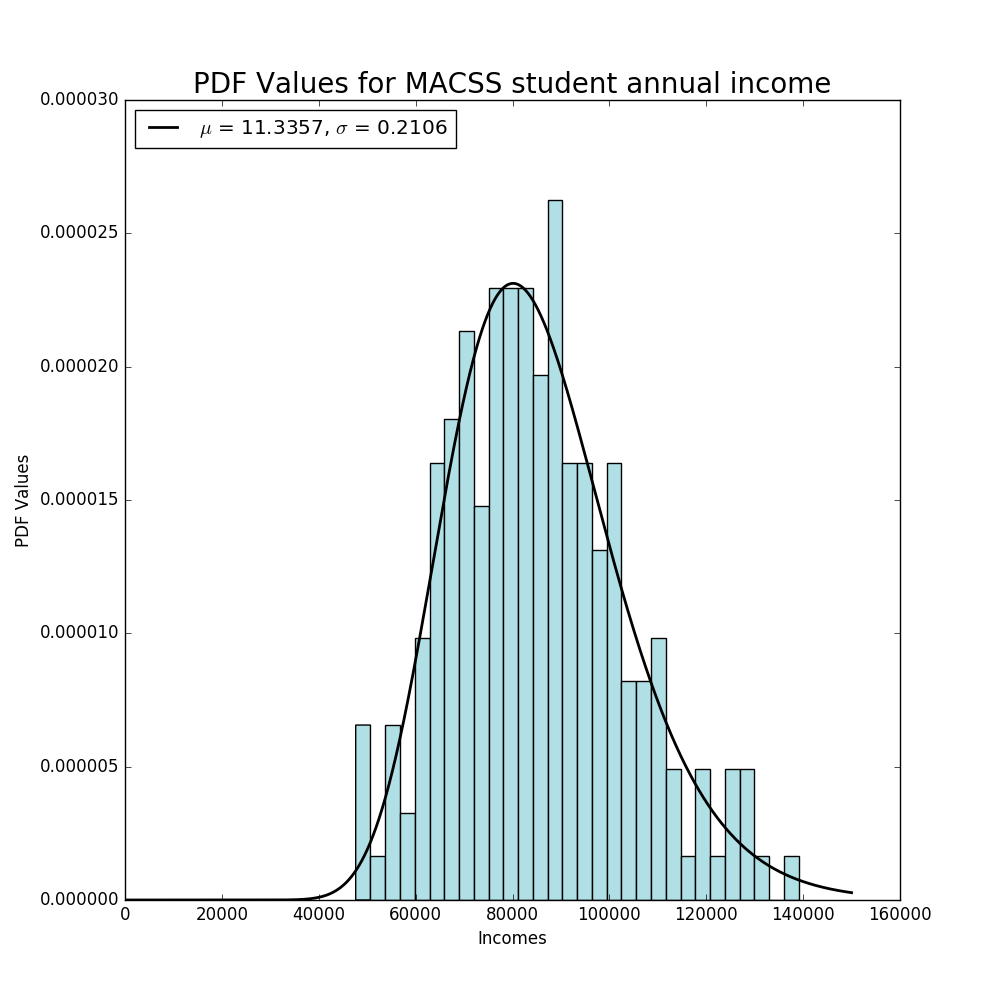
\includegraphics{Fig_1d.png}}}
\end{figure}
\\
\noindent\textbf{Part (e).}\\
\begin{figure}[htb]\centering\captionsetup{width=4.0in}
  \label{Fig1e}
  \fbox{\resizebox{4.0in}{3.0in}{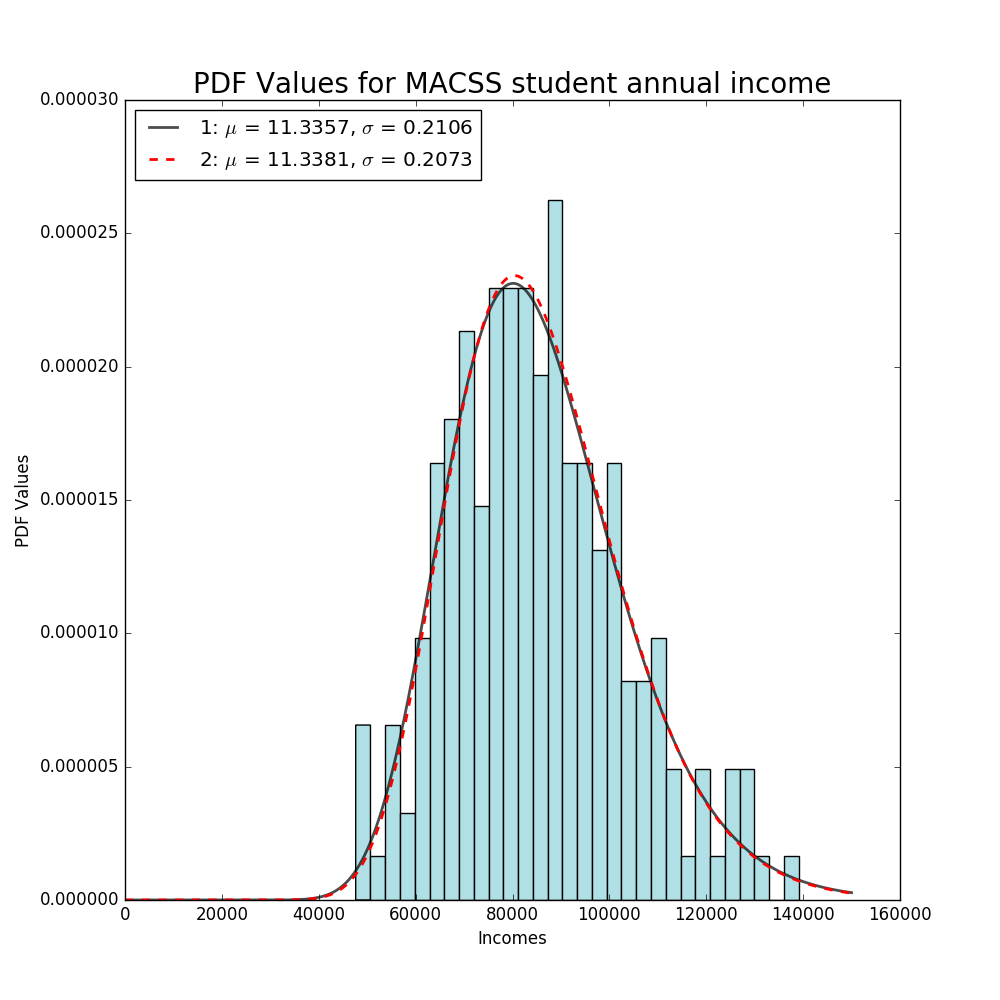
\includegraphics{Fig_1e.png}}}
\end{figure}
\\
The value of GMM criterion function at the estimated parameter values is: \\
$91.95874552987516$.\\
The three data moments are: \\
the proportion of individuals who earn less than \$75,000 is: $0.3$, \\
the proportion of individuals who earn more than \$75,000 but less than \$100,000 is: $0.5$, \\
the proportion of individuals who earn more than \$100,000 is: $0.2$. \\
The three model moments are: \\
the proportion of individuals who earn less than \$75,000 is: $0.2931$, \\
the proportion of individuals who earn more than \$75,000 but less than \$100,000 is: $0.5073$, \\
the proportion of individuals who earn more than \$100,000 is: $0.1996$.\\
Outcomes from 2-step GMM seems less close to data moments.\\
\\
\noindent\textbf{Part (f).}\\
From the above five figures, we could see that lognormal pdf figure in fig b, d, and e seem to fit the histogram i.e. our data well. Among these three pdf, the pdf generated from 2-step GMM with three data moments (Fig 1e) seems the best to me. This pdf has slightly thinner left tail and higher peak in the middle, which seems to be the feature of this income data set.\\
\\
\noindent\textbf{Problem 2. Linear regression and GMM.}\\
\\
\noindent\textbf{Part (a).}\\
\\
$\beta^{ggm}_{0} = .2516\quad \beta^{ggm}_{1} = 0.0129\quad\beta^{ggm}_{2} = 0.4005\quad \beta^{ggm}_{3} = -0.0100\quad$
\\
The value of GMM criterion function is: $0.001821$.\\
\end{document}
